\documentclass[12pt]{article}
\usepackage[utf8]{inputenc}
\usepackage[spanish]{babel}
\usepackage{graphicx}
\usepackage{amsmath}
\usepackage{amssymb}
\usepackage{array}
\usepackage{xcolor}
\usepackage{geometry}
\usepackage{fancyhdr}
\usepackage{lastpage}
\usepackage{booktabs}
\usepackage{colortbl}
\usepackage{caption}
\usepackage{multirow}
\geometry{margin=1in}

\usepackage{float}
\definecolor{lightblue}{RGB}{200,230,255}
\definecolor{lightgreen}{RGB}{220,255,220}
\definecolor{lightred}{RGB}{255,220,220}
\definecolor{lightyellow}{RGB}{255,255,200}
\pagestyle{fancy}
\fancyhf{}
\fancyhead[L]{Algoritmo de Floyd - Solución}
\fancyhead[R]{\thepage\ de \pageref{LastPage}}
\renewcommand{\headrulewidth}{0.4pt}
\renewcommand{\footrulewidth}{0.4pt}

\title{Proyecto 1: Rutas Optimas (Algoritmo de Floyd)}
\author{Emily Sanchez \\ Viviana Vargas \\[1cm] Curso: Investigación de Operaciones \\ II Semestre 2025}
\date{\today}

\begin{document}

\maketitle
\thispagestyle{empty}
\newpage
\setcounter{page}{1}

\section{Introducción}
El algoritmo de Floyd-Warshall es un algoritmo para encontrar los caminos más cortos en un grafo ponderado. Fue publicado por Robert Floyd en 1962.\\
El algoritmo de Floyd se basa en el principio de la Programación Dinámica.\\
\textbf{Complejidad espacial:} $O(n^2)$\\
\textbf{Complejidad temporal:} $O(n^3)$\\
\clearpage
\section{Descripción del Problema}
Grafo con 4 nodos:

\begin{itemize}
\item Nodo A: A
\item Nodo B: B
\item Nodo C: C
\item Nodo D: D
\end{itemize}

\begin{figure}[h!]
\centering
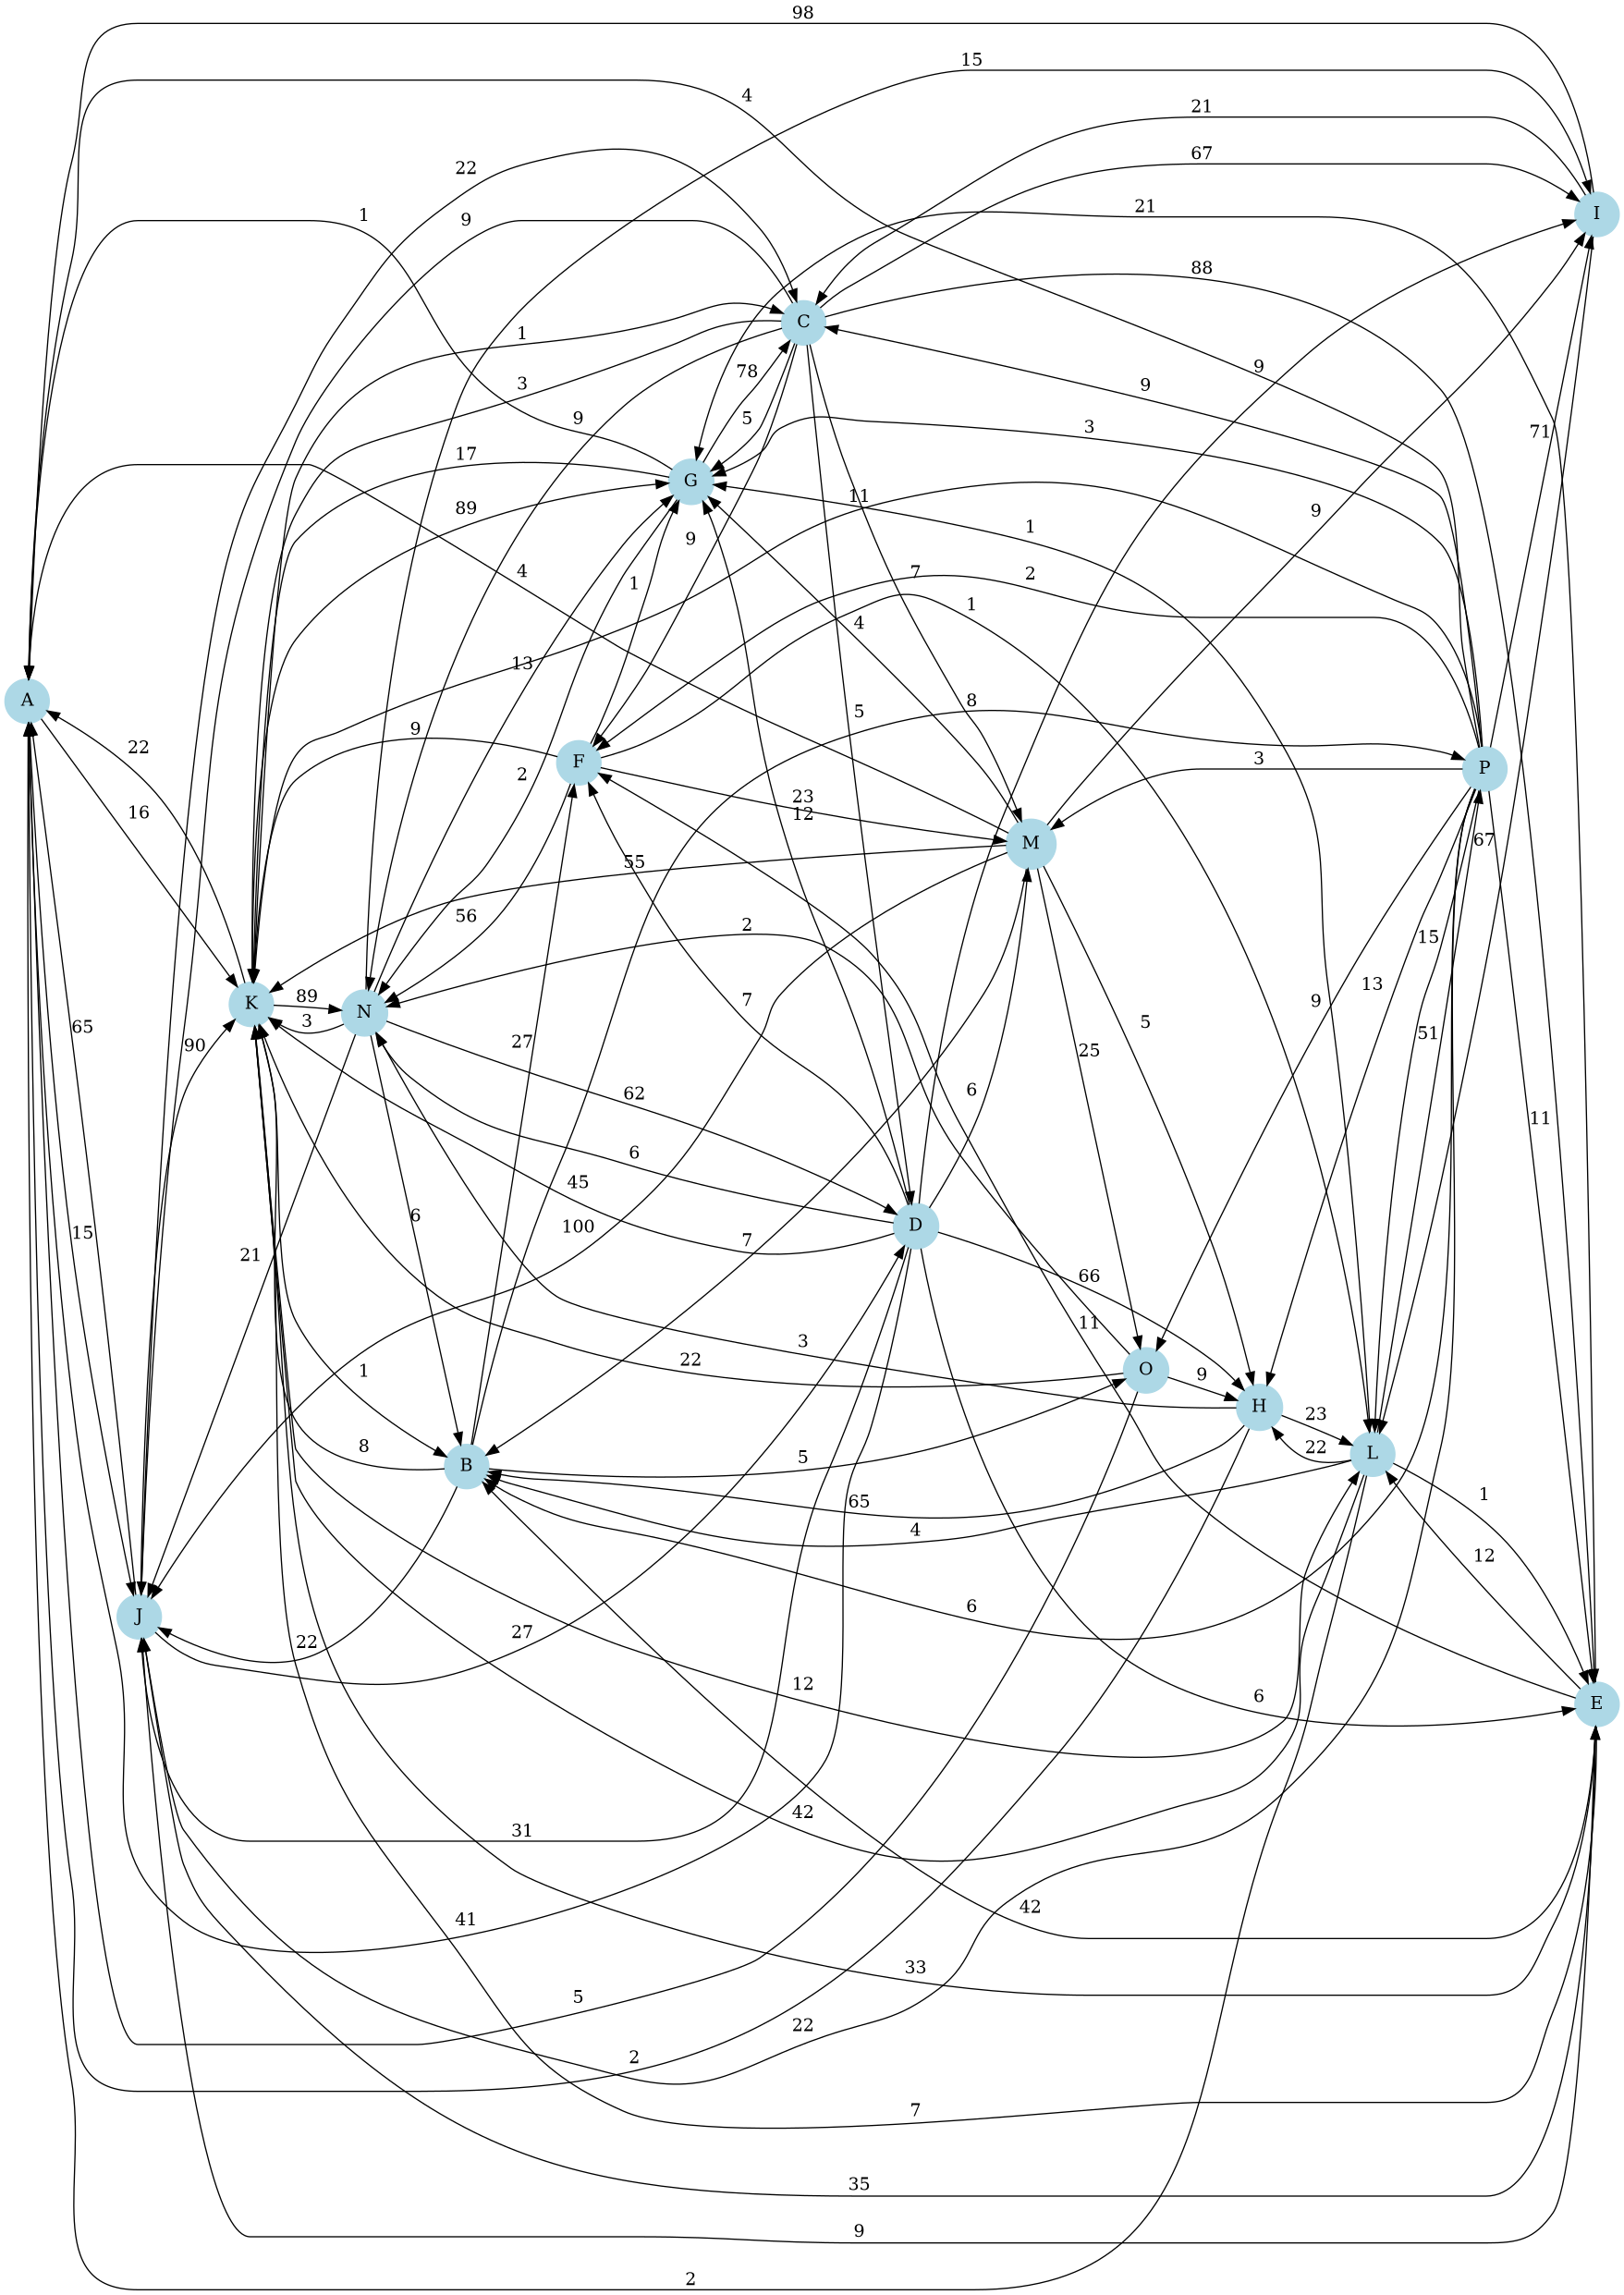
\includegraphics[width=0.5\textwidth,keepaspectratio]{grafo.png}
\caption{Representación del grafo original}
\end{figure}

\clearpage
\section{Procedimiento del Algoritmo}
\subsection{Matriz de Distancias Inicial D(0)}
\begin{table}[h!]
\centering
\begin{tabular}{|c|c|c|c|c|}
\hline
 & A & B & C & D \\\hline
A & 0 & 15 & 12 & 1 \\\hline
B & $\infty$ & 0 & $\infty$ & $\infty$ \\\hline
C & 12 & 6 & 0 & 15 \\\hline
D & 2 & $\infty$ & 11 & 0 \\\hline
\end{tabular}
\caption{Matriz de distancias inicial D(0)}
\end{table}

\clearpage
\subsection{Matriz de Caminos Inicial P(0)}
\begin{table}[h!]
\centering
\begin{tabular}{|c|c|c|c|c|}
\hline
 & A & B & C & D \\\hline
A & - & A & A & A \\\hline
B & - & - & - & - \\\hline
C & C & C & - & C \\\hline
D & D & - & D & - \\\hline
\end{tabular}
\caption{Matriz de caminos inicial P(0)}
\end{table}

\clearpage
\subsection{Iteraciones del Algoritmo}
\clearpage
\subsubsection{Iteración 1 (k = 1) - Nodo intermedio: A}
\paragraph{Matriz de Distancias D(1)}
\begin{table}[h!]
\centering
\begin{tabular}{|c|c|c|c|c|}
\hline
 & A & B & C & D \\\hline
A & 0 & 15 & 12 & 1 \\\hline
B & $\infty$ & 0 & $\infty$ & $\infty$ \\\hline
C & 12 & 6 & 0 & \cellcolor{lightgreen} 13 \\\hline
D & 2 & \cellcolor{lightgreen} 17 & 11 & 0 \\\hline
\end{tabular}
\caption{Matriz de distancias D(1) - Cambios resaltados en verde}
\end{table}

\paragraph{Matriz de Caminos P(1)}
\begin{table}[h!]
\centering
\begin{tabular}{|c|c|c|c|c|}
\hline
 & A & B & C & D \\\hline
A & - & A & A & A \\\hline
B & - & - & - & - \\\hline
C & C & C & - & \cellcolor{lightblue} A \\\hline
D & D & \cellcolor{lightblue} A & D & - \\\hline
\end{tabular}
\caption{Matriz de caminos P(1) - Cambios resaltados en azul}
\end{table}

\clearpage
\subsubsection{Iteración 2 (k = 2) - Nodo intermedio: B}
\paragraph{Matriz de Distancias D(2)}
\begin{table}[h!]
\centering
\begin{tabular}{|c|c|c|c|c|}
\hline
 & A & B & C & D \\\hline
A & 0 & 15 & 12 & 1 \\\hline
B & $\infty$ & 0 & $\infty$ & $\infty$ \\\hline
C & 12 & 6 & 0 & 13 \\\hline
D & 2 & 17 & 11 & 0 \\\hline
\end{tabular}
\caption{Matriz de distancias D(2) - Cambios resaltados en verde}
\end{table}

\paragraph{Matriz de Caminos P(2)}
\begin{table}[h!]
\centering
\begin{tabular}{|c|c|c|c|c|}
\hline
 & A & B & C & D \\\hline
A & - & A & A & A \\\hline
B & - & - & - & - \\\hline
C & C & C & - & A \\\hline
D & D & A & D & - \\\hline
\end{tabular}
\caption{Matriz de caminos P(2) - Cambios resaltados en azul}
\end{table}

\clearpage
\subsubsection{Iteración 3 (k = 3) - Nodo intermedio: C}
\paragraph{Matriz de Distancias D(3)}
\begin{table}[h!]
\centering
\begin{tabular}{|c|c|c|c|c|}
\hline
 & A & B & C & D \\\hline
A & 0 & 15 & 12 & 1 \\\hline
B & $\infty$ & 0 & $\infty$ & $\infty$ \\\hline
C & 12 & 6 & 0 & 13 \\\hline
D & 2 & 17 & 11 & 0 \\\hline
\end{tabular}
\caption{Matriz de distancias D(3) - Cambios resaltados en verde}
\end{table}

\paragraph{Matriz de Caminos P(3)}
\begin{table}[h!]
\centering
\begin{tabular}{|c|c|c|c|c|}
\hline
 & A & B & C & D \\\hline
A & - & A & A & A \\\hline
B & - & - & - & - \\\hline
C & C & C & - & A \\\hline
D & D & A & D & - \\\hline
\end{tabular}
\caption{Matriz de caminos P(3) - Cambios resaltados en azul}
\end{table}

\clearpage
\subsubsection{Iteración 4 (k = 4) - Nodo intermedio: D}
\paragraph{Matriz de Distancias D(4)}
\begin{table}[h!]
\centering
\begin{tabular}{|c|c|c|c|c|}
\hline
 & A & B & C & D \\\hline
A & 0 & 15 & 12 & 1 \\\hline
B & $\infty$ & 0 & $\infty$ & $\infty$ \\\hline
C & 12 & 6 & 0 & 13 \\\hline
D & 2 & 17 & 11 & 0 \\\hline
\end{tabular}
\caption{Matriz de distancias D(4) - Cambios resaltados en verde}
\end{table}

\paragraph{Matriz de Caminos P(4)}
\begin{table}[h!]
\centering
\begin{tabular}{|c|c|c|c|c|}
\hline
 & A & B & C & D \\\hline
A & - & A & A & A \\\hline
B & - & - & - & - \\\hline
C & C & C & - & A \\\hline
D & D & A & D & - \\\hline
\end{tabular}
\caption{Matriz de caminos P(4) - Cambios resaltados en azul}
\end{table}

\clearpage
\section{Resultados Finales}
\subsection{Matriz de Distancias Final D(4)}
\begin{table}[h!]
\centering
\begin{tabular}{|c|c|c|c|c|}
\hline
 & A & B & C & D \\\hline
A & 0 & 15 & 12 & 1 \\\hline
B & $\infty$ & 0 & $\infty$ & $\infty$ \\\hline
C & 12 & 6 & 0 & 13 \\\hline
D & 2 & 17 & 11 & 0 \\\hline
\end{tabular}
\caption{Matriz de distancias final D(4)}
\end{table}

\clearpage
\subsection{Matriz de Caminos Final P(4)}
\begin{table}[h!]
\centering
\begin{tabular}{|c|c|c|c|c|}
\hline
 & A & B & C & D \\\hline
A & - & A & A & A \\\hline
B & - & - & - & - \\\hline
C & C & C & - & A \\\hline
D & D & A & D & - \\\hline
\end{tabular}
\caption{Matriz de caminos final P(4)}
\end{table}

\clearpage
\subsection{Rutas Óptimas}
\begin{itemize}
\item \textbf{A → B:} Distancia: 15, Ruta: A → B
\item \textbf{A → C:} Distancia: 12, Ruta: A → C
\item \textbf{A → D:} Distancia: 1, Ruta: A → D
\item \textbf{C → A:} Distancia: 12, Ruta: C → A
\item \textbf{C → B:} Distancia: 6, Ruta: C → B
\item \textbf{C → D:} Distancia: 13, Ruta: C → A → D
\item \textbf{D → A:} Distancia: 2, Ruta: D → A
\item \textbf{D → B:} Distancia: 17, Ruta: D → A → B
\item \textbf{D → C:} Distancia: 11, Ruta: D → C
\end{itemize}
\end{document}
